\documentclass[10pt]{beamer}
% Class options include: notes, notesonly, handout, trans,
%                        hidesubsections, shadesubsections,
%                        inrow, blue, red, grey, brown

% Theme for beamer presentation.
%\usepackage{beamerthemelined} 
%\usepackage{times}
\usepackage{anysize}
\usepackage{fancyhdr}
\usepackage{graphicx}
\usepackage{pdfpages}
\usepackage{amsmath}
\usepackage{amssymb}
\usepackage{hyperref}
 \hypersetup{
 colorlinks=true,
 linkcolor=black
 }
% Other themes include: beamerthemebars, beamerthemelined, 
%                       beamerthemetree, beamerthemetreebars  

\title{\bfseries Term Indexing for the \\ Beagle Theorem Prover}    % Enter your title between curly braces
\author{Tim Cosgrove \vspace{-0.3cm}}                 % Enter your name between curly braces
\institute{COMP4006 Honours Research Project \\ \vspace{0.3cm}
Research School of Computer Science,\\
Australian National University \\ \vspace{0.3cm}
\texttt{u4843619@anu.edu.au} \\ \vspace{0.3cm}
Supervisor: Peter Baumgartner}      % Enter your institute name between curly braces
\date{\today}                    % Enter the date or \today between curly braces

\usetheme{Hannover}
\usecolortheme{orchid}
\setbeamertemplate{navigation symbols}{}

\newcommand{\bcen}{\begin{center}}
\newcommand{\ecen}{\end{center}}
\newcommand{\HSWAC}{Hierarchic Superposition with Weak Abstraction Calculus}
\newcommand{\HSWA}{Hierarchic Superposition with Weak Abstraction}

\begin{document}

\begin{NoHyper}
% Creates title page of slide show using above information
\begin{frame}
  \titlepage
\end{frame}
\note{} % Add notes to yourself that will be displayed when
        % typeset with the notes or notesonly class options

\section[Outline]{}

% Creates table of contents slide incorporating
% all \section and \subsection commands
\begin{frame}
  \tableofcontents
\end{frame}
%%%%%%%%%%%%%%%%%%%%%%%%%%%%%%%%%%%%%%%%%%%%%%%%%%%%%%%%%%%%%%%%%%%%%%%%%%%%%%%%
\section{Project Overview}
%%%%%%%%%%%%%%%%%%%%%%%%%%%%%%%%%%%%%%%%%%%%%%%%%%%%%%%%%%%%%%%%%%%%%%%%%%%%%%%%

\subsection{Motivation}

%%%%%%%%%%%%%%%%%%%%%%%%%%%%%%%%%%%%%%%%%%%%%%%%%%%%%%%%%%%%%%%%%%%%%%%%%%%%%%%%
\section{Background}
%%%%%%%%%%%%%%%%%%%%%%%%%%%%%%%%%%%%%%%%%%%%%%%%%%%%%%%%%%%%%%%%%%%%%%%%%%%%%%%%

%%%%%%%%%%%%%%%%%%%%%%%%%%
\subsection{The Beagle Theorem Prover}
%%%%%%%%%%%%%%%%%%%%%%%%%%

\begin{frame}
  \frametitle{The Beagle Theorem Prover}
  \begin{itemize}
  \item<1-> Beagle is a First-Order-Logic resolution theorem prover with equality.
  \item<2-> Makes use of modular 'Background Theories' to make efficient use of known facts.
  \item<3-> This requires the carefully constructed `Hierarchic Superposition with Weak Abstraction
  Calculus' in order to ensure consistency and completeness.
  \end{itemize}
\end{frame}

\begin{frame}
  \frametitle{Superposition Calculus}
  \begin{itemize}
  \item<1-> Normal Superposition rule
  \end{itemize}
\end{frame}

\begin{frame}
  \frametitle{\HSWAC}
  \begin{itemize}
  \item<1-> Extension of Superposition Calculus to accommodate hierarchic reasoning.
  \end{itemize}
\end{frame}

%%%%%%%%%%%%%%%%%%%%%%%%%%
\subsection{Term Indexing} 
%%%%%%%%%%%%%%%%%%%%%%%%%%
\begin{frame}
  \frametitle{Term Indexing Techniques}
  \begin{itemize}
  \item<1-> Term indexers aim to collect all FOL terms which potentially match a `query' term.
  \item<1-> Three important relations:
  \begin{itemize}
  \item<2-> 'Unifiable': $\sigma s = \sigma t$
  \item<2-> 'Instance Of': $s = \sigma t$
  \item<2-> 'Generalises': $\sigma s = t$
  \end{itemize}
  \item<3-> Top-Symbol Hashing.
  \item<3-> Discrimination Trees.
  \item<3-> Path Indexing.
  \end{itemize}
\end{frame}

%%%%%%%%%%%%%%%%%%%%%%%%%%
\subsection{Fingerprint Indexing} 
%%%%%%%%%%%%%%%%%%%%%%%%%%
\begin{frame}
  \frametitle{Fingerprint Indexing}
                  %Left Bot Right Top
  \begin{itemize}
  \item<1-> Maintain a collection of \emph{fingerprints} for terms.
  \item<2-> A term fingerprint is an array over $F \cup \{\mathbf{A, B, N}\}$.
  \item<3-> \includegraphics[page=6,scale=0.7,trim=5.5cm 20.5cm 5cm 4cm,clip]{schulz_fp-index_ext}
  \item<4-> {\footnotesize Schulz, Stephan: Fingerprint Indexing for Paramodulation and Rewriting. In:
  Lecture Notes in Computer Science volume 7364 pp. 447--483 (2012).}

  \end{itemize}
\end{frame}

  \begin{frame}
  \frametitle{Fingerprint Indexing -- Potential Performance}
  \begin{center}{\tiny
  \begin{tabular}{| l | r | r | r | r | r | r | r |} \hline
  Index & Run time & Sat time & PM time & PMI time & MGU time & BR time & BRI time \\ \hline
NoIdx & 16062.392 & 14078.300 &  8980.320 & 0.000 & 2545.080  & 2280.250 & 0.000\\
FP1 & 7006.758 & 6145.870 & 1816.100 & 25.710 & 450.760 & 379.570 & 40.150\\
FP6M & 6000.177 & 5385.810 & 1181.710 & 38.240 & 99.110 & 39.010 & 55.660\\
NPDT & 6082.246 & 5434.760 & 1184.750 & 64.910 & 83.110 & 33.200 & 79.910 \\\hline
  \end{tabular}}\vspace{0.5cm}
                  %Left Bot Right Top
  \includegraphics[page=13,scale=0.5,trim=6cm 8cm 7cm 12cm,clip]{schulz_fp-index_ext}
  \hspace{1cm}
                  %Left Bot Right Top
  \includegraphics[page=14,scale=0.5,trim=6cm 16.2cm 7cm 4cm,clip]{schulz_fp-index_ext}
  \end{center}
\end{frame}

%\begin{frame}
%  \frametitle{Fingerprint Indexing -- Example Fingerprint Index}
   %Structure of fingerprint indexes
                  %Left Bot Right Top
%  \includegraphics[page=7,scale=0.7,trim=4cm 13.5cm 5cm 4.5cm,clip]{schulz_fp-index_ext}
%\end{frame}
%%%%%%%%%%%%%%%%%%%%%%%%%%%%%%%%%%%%%%%%%%%%%%%%%%%%%%%%%%%%%%%%%%%%%%%%%%%%%%%%
\section{Implementation}
%%%%%%%%%%%%%%%%%%%%%%%%%%%%%%%%%%%%%%%%%%%%%%%%%%%%%%%%%%%%%%%%%%%%%%%%%%%%%%%%

%%%%%%%%%%%%%%%%%%%%%%%%%%
\subsection{Implementing Fingerprint Indexing}
%%%%%%%%%%%%%%%%%%%%%%%%%%
\begin{frame}
  \frametitle{Base Fingerprint Indexing}
                  %Left Bot Right Top
  \begin{itemize}
  \item<1-> Analysis of program indicated two key areas of improvement:
  \item<2-> Inferences via the Superposition rules.
  \item<2-> Simplifying Clauses.
  \end{itemize}
\end{frame}

\begin{frame}
  \frametitle{Creating the Fingerprint Index}
  \begin{itemize}
  \item<1-> Addition of terms.
  \item<2-> Retrieval of terms.
  \end{itemize}
\end{frame}

%%%%%%%%%%%%%%%%%%%%%%%%%%
\subsection{Indexing Applications}
%%%%%%%%%%%%%%%%%%%%%%%%%%
\begin{frame}
  \frametitle{Indexing Superposition}
  \begin{itemize}
  \item<1-> Refer to rule. Requires...
  \end{itemize}
\end{frame}

\begin{frame}
  \frametitle{Indexing Simplification}
  \begin{itemize}
  \item<1-> Refer to rule. Requires...
  \end{itemize}
\end{frame}

%%%%%%%%%%%%%%%%%%%%%%%%%%
\subsection{Tailoring to Beagle}
%%%%%%%%%%%%%%%%%%%%%%%%%%
\begin{frame}
  \frametitle{Fingerprint Indexing for the Hierarchic Superposition with Weak Abstraction Calculus}
                  %Left Bot Right Top
  \begin{itemize}
  \item<1-> As mentioned, current implementation is somewhat `na\"{i}ve'.
  \item<2-> Fingerprint indexing could be greatly improved by tailoring it specifically
  to Beagle's FOL calculus.
  \item<2-> Main improvement is to consider Beagle's \emph{foreground} and \emph{background}
  terms.
  \item<3-> Furthermore indexing may be applied to more
  of HSWA's inference rules; in particular simplification.
  \item<4-> These extensions will not require so much modification; as the fingerprint
  indexing framework is already built.
  \end{itemize}
\end{frame}

%%%%%%%%%%%%%%%%%%%%%%%%%%
\subsection{Other Improvements}
%%%%%%%%%%%%%%%%%%%%%%%%%%
\begin{frame}
  \frametitle{Other Potential Indexing Improvements}
  \begin{itemize}
  \item<1-> An additional goal of the project is to consider how Fingerprint Indexing
  could be improved upon more generally.
  \item<2-> The main area to consider here is the sampling positions. Sampling many
  positions reduces the returned sets, but increases indexing overhead.
  \item<3-> Large problems better suit indexing; but it is difficult to know ahead of
  time what a `large' problem is.
  \end{itemize}
\end{frame}



%%%%%%%%%%%%%%%%%%%%%%%%%%%%%%%%%%%%%%%%%%%%%%%%%%%%%%%%%%%%%%%%%%%%%%%%%%%%%%%%
\section{Results}
%%%%%%%%%%%%%%%%%%%%%%%%%%%%%%%%%%%%%%%%%%%%%%%%%%%%%%%%%%%%%%%%%%%%%%%%%%%%%%%%

%%%%%%%%%%%%%%%%%%%%%%%%%%
\subsection{Evaluation Metrics}
%%%%%%%%%%%%%%%%%%%%%%%%%%
\begin{frame}
  \begin{itemize}
  \frametitle{Metrics for Analysing Indexing Performance}
  \item<1-> Speed - Not necessarily relevant
  \item<2-> False Positives - Relevant, but can be misleading depending on
  number of positions being sampled.
  \item<3-> Time Spent \emph{per Inference} - Booyah
  \end{itemize}
\end{frame}


%%%%%%%%%%%%%%%%%%%%%%%%%%
\subsection{Beagle Comparisons}
%%%%%%%%%%%%%%%%%%%%%%%%%%
\begin{frame}
  \begin{itemize}
  \frametitle{Comparing Varieties of Beagle}
  \item<1-> Un-indexed beagle.
  \item<2-> Minimal Indexing.
  \item<3-> Full Indexing.
  \item<4-> Indexing with Optimisations.
  \end{itemize}
\end{frame}

\begin{frame}
  \begin{itemize}
  \frametitle{Comparing Varieties of Beagle}
  \item<1-> Results table
  \end{itemize}
\end{frame}

\begin{frame}
  \begin{itemize}
  \frametitle{Most Extreme Example Problems}
  \item<1-> Describe crazy DAT results.
  \end{itemize}
\end{frame}

%%%%%%%%%%%%%%%%%%%%%%%%%%
\subsection{Sample Position Comparisons}
%%%%%%%%%%%%%%%%%%%%%%%%%%
\begin{frame}
  \begin{itemize}
  \frametitle{Fingerprint Sampling Varieties}
  \item<1-> Reasoning. Cite shulz and FP/Speed balance
  \item<2-> Different position samples
  \end{itemize}
\end{frame}

\begin{frame}
  \begin{itemize}
  \frametitle{Fingerprint Sampling Varieties}
  \item<1-> Results table
  \end{itemize}
\end{frame}

%%%%%%%%%%%%%%%%%%%%%%%%%%%%%%%%%%%%%%%%%%%%%%%%%%%%%%%%%%%%%%%%%%%%%%%%%%%%%%%%
\section{Conclusion}
%%%%%%%%%%%%%%%%%%%%%%%%%%%%%%%%%%%%%%%%%%%%%%%%%%%%%%%%%%%%%%%%%%%%%%%%%%%%%%%%



\end{NoHyper}
\end{document}
